\documentclass[conference]{IEEEtran}
% *** GRAPHICS RELATED PACKAGES ***
%
\ifCLASSINFOpdf
  \usepackage[pdftex]{graphicx}
  % declare the path(s) where your graphic files are
  % \graphicspath{{../pdf/}{../jpeg/}}
  % and their extensions so you won't have to specify these with
  % every instance of \includegraphics
  \DeclareGraphicsExtensions{.pdf,.jpeg,.png}
\else
  % or other class option (dvipsone, dvipdf, if not using dvips). graphicx
  % will default to the driver specified in the system graphics.cfg if no
  % driver is specified.
  \usepackage[dvips]{graphicx}
  % declare the path(s) where your graphic files are
  % \graphicspath{{../eps/}}
  % and their extensions so you won't have to specify these with
  % every instance of \includegraphics
  % \DeclareGraphicsExtensions{.eps}
\fi

\usepackage{pgf}
%\usepackage{tikz}
%\usetikzlibrary{arrows,automata}

\definecolor{darkgreen}{rgb}{0,0.7,0}

\newif\ifdraft
\drafttrue
%\draftfalse
\ifdraft
 \newcommand{\katznote}[1]{ {\textcolor{blue} { ***Dan:   #1 }}}
 \newcommand{\ketanote}[1]{{\textcolor{orange}  { ***Ketan:   #1 }}}
 \newcommand{\kriedernote}[1]{ {\textcolor{darkgreen}  { ***Scott:   #1 }}}
 \newcommand{\note}[1]{ {\textcolor{red}    {\bf #1 }}}
\else
 \newcommand{\katznote}[1]{}
 \newcommand{\kriedernote}[1]{}
 \newcommand{\note}[1]{}
\fi
% correct bad hyphenation here
%\hyphenation{op-tical net-works semi-conduc-tor}

\hyphenation{Queuing}

\begin{document}
%
% can use linebreaks \\ within to get better formatting as desired
\title{Understanding the Costs of Many-Task Computing Workloads on Intel Xeon Phi Coprocessors}

%\author{\IEEEauthorblockN{Auth1\IEEEauthorrefmark{1},
%Auth2\IEEEauthorrefmark{1}\IEEEauthorrefmark{1}, 
%Auth3\IEEEauthorrefmark{1},
%\IEEEauthorblockA{\IEEEauthorrefmark{1}Argonne National Laboratory}
%}}

\author{Jeffrey Johnson\IEEEauthorrefmark{1},
Scott J. Krieder\IEEEauthorrefmark{1},
Benjamin Grimmer\IEEEauthorrefmark{1}\\
Justin M. Wozniak\IEEEauthorrefmark{2},
Michael Wilde\IEEEauthorrefmark{2}\IEEEauthorrefmark{3},
Ioan Raicu\IEEEauthorrefmark{1}\IEEEauthorrefmark{2}\\
\IEEEauthorblockA{
\IEEEauthorrefmark{1}Department of Computer Science, Illinois Institute of Technology}
\IEEEauthorrefmark{2}MCS Division, Argonne National Laboratory\\
\IEEEauthorrefmark{3}Computation Institute, University of Chicago
}


\maketitle


\begin{abstract}
Many-Task Computing (MTC) aims to bridge the gap between HPC and HTC. MTC emphasizes running many computational tasks over a short period of time, where tasks can be either dependent or independent of one another. MTC has been well supported on Clouds, Grids, and Supercomputers on traditional computing architectures, but the abundance of hybrid large-scale systems using accelerators has motivated us to explore the support of MTC on the new Intel Xeon Phi accelerators. The Xeon Phi is a PCI-Express based expansion card comprised of 60 cores supporting 240 hardware threads to produce up to 1 teraflop of double- precision performance in a single accelerator. These cards are already being integrated into super-computing clusters such as Stampede which hosts over 6,400 Xeon Phi Accelerators totaling in over 7 petaflops of double- precision performance. This work provides an in depth understanding of MTC on the Intel Xeon Phi and presents our preliminary results of running several different workloads on pre-production Intel Xeon Phi hardware. By utilizing Intel’s provided SCIF protocol for communicating across the PCI-Express bus we have achieved over 90\% efficiency near or outperforming OpenMP offloading tasks over 300 uS with our batch framework. This performance opens the opportunity for the development of a framework for executing heterogeneous tasks on the Xeon Phi alongside other potential accelerators including graphics cards for MTC applications. Our framework will provide fine granularity for executing MTC applications across large scale compute clusters. It will be integrated with our existing graphics card framework, GemTC, to provide transparent access to GPU’s, Xeon Phi’s, and future generations of accelerators to help bridge the gap into exascale computing
\end{abstract}

% no keywords
\begin{IEEEkeywords}
MIMD, MTC, Accelerator, Intel Xeon Phi, Coprocessor
\end{IEEEkeywords}

\IEEEpeerreviewmaketitle

\section{Introduction}
In this work we provide preliminary results evaluating MTC workloads running on Intel Xeon Phi Coprocessors. The Intel Xeon Phi Coprocessor is physically similar to other hardware accelerators such as GPGPUs but contains many significant underlying differences.

The High Performance Computing (HPC) community is seeing a large adaptation of general-purpose accelerator cards. In the past years [X], graphics cards have become a significant part of newly built computing clusters providing unprecedented parallelism with a low power footprint. Accelerators often require the use of reworking a program in order to use or fully utilize the device and as a result increase development time.

The pre-production Xeon Phi is a 61-core accelerator featuring 8 GB of GDDR5 connected to the host via a PCI Express bus. The Phi runs an instance of the Linux operating system, which occupies a single core of the accelerator to provide the developer with a familiar programming interface. As of the pre- production Xeon Phi, it is possible to use OpenMP, POSIX threads, OpenCL, Intel Math Kernel Library, MPI, or other popular libraries to develop and offload applications to the accelerator. Intel also provides a socket protocol, SCIF, to aid in data transfer between the host and the Phi to transfer data across the PCI Express bus. Intel also provides the application ‘micnativeloadex’ to launch an application compiled for the Phi on the accelerator. This application ensures the correct libraries and program code are copied and executed on the accelerator.

\section{Architecture}
In order to provide a seamless and easy to use interface, our framework sets out to provides identical functionality to GeMTC. \cite{kriederSC12} GeMTC has three types off operations: Push/Pool for sending and receiving jobs, Malloc/Free for preparing device memory, and a memory copy operation to copy data to or from the accelerator. By providing this interface we can easily tie in with Swift/T to open up our solution to multi-node configurations.

\subsection{SCIF Implementation}
Our SCIF framework employs a client server architecture, which communicates via the Symmetric Communications Interface (SCIF). This interface abstracts communication across the PCI- Express bus to a UNIX socket semantics. The server application uses a single process launched on the Intel Xeon Phi, which then launches a single processing thread per hardware core to handle incoming work from the host. The client starts from a single process and launches no more threads than the server. Each server thread listens via SCIF on a discrete port, which is used to accept and return work to the client. Each client thread produces a batch of work to the accelerator, which can contain a heterogeneous list of tasks with varying lengths and data payload sizes. The client blocks until the entire batch is completed. This architecture allows the overhead of launching threads as well as offloading the code to be executed to be ignored and performance becomes only dependent on data transfer rate and processing rate of the processor. This framework does not provide the feature set of GeMTC due to the complexity of data transfer between the device and host over SCIF. Each party in the communication is forced to manually parse out received streams of data which is a highly error prone operation when dealing with complex lists of tasks.

\section{Preliminary Results}
In this section we present preliminary results for running several synthetic benchmarks on pre-production Intel Xeon Phi hardware.

\subsection{Synthetic Sleep Workloads}
To compare the overhead of our architecture with OpenMP three sleep programs are analyzed. The first uses our SCIF framework to launch a batch of sleep jobs to the Xeon Phi and block until completion then separately tests launching individual jobs to the device and waiting for the result before pushing the next job. The second uses OpenMP to offload a single block, which calls a sleep job 128 times by repetitively placing the function call in the block. This method was chosen to more accurately mimic the loop-unrolling style of our SCIF framework. The final program uses OpenMP to offload a single sleep task and is repeatedly called. Figure \ref{fig:sleep_phi}demonstrates the results of comparing all four different configurations in varying sleep lengths. By testing varying lengths of sleeps, we find that jobs over 320 uS benefit from the SCIF framework when sent in this length of a batch. At this point the performance is slightly above OpenMP but can enjoy the potential benefits of the framework.

\section{Related Work}
The Xeon Phi is a very new technology and research is just beginning to show the usefulness of the technology. IRWTH Aachen University and Intel have collaborated on a paper outlining the initial performance of the preproduction Xeon Phi demonstrating the power of its dense processing using OpenMP related to a traditional 128-core system. It was shown that a single Phi had a lower overall performance but the power per core and power efficiency significantly outweighs the latter solution towards many-core. Intel also advocates the offloading capabilities of its compiler and OpenMP with use of the Phi showing that many OpenMP programs can be launched on the Phi without code change.

\section{Conclusions and Future Work}
It has been demonstrated that is it possible to achieve minimum overhead with the Xeon Phi by directly communicating between the host and accelerator via SCIF across the PCI Express bus. Using our proposed framework, it will be possible to share the resources of a Xeon Phi across multiple processes and users in a large scale computing environment while maintaining high performance through the use of specialized microkernels. Enabling the Xeon Phi to run heterogeneous workloads can enable the device to be used in a Many-Task Computing \cite{raicu2008toward} environment where resources are shared between users and latency is important. The findings of this paper shows no significant performance tradeoff to the framework opening the way for a promising use of the Xeon Phi in new environments.

\begin{figure}[h]
\centering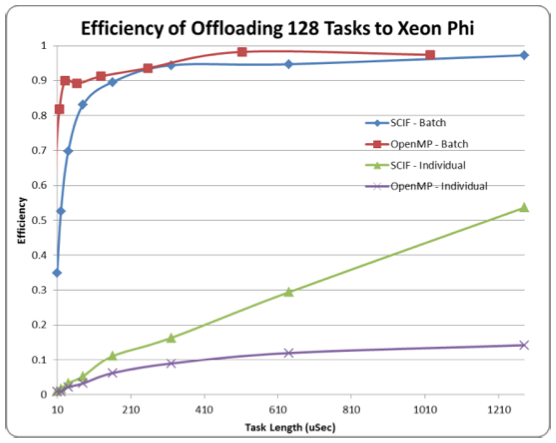
\includegraphics[width=8cm]{imgs/sleep_phi.png}
\caption{Efficiency of Offloading 128 Tasks to Xeon Phi Comparison between OpenMP and SCIF with individual offloads and batch offloads.}
\label{fig:sleep_phi}
\end{figure}

\bibliographystyle{IEEEtran}
\bibliography{ref}
\end{document}
